%% TESS Director's Discretionary Targets proposal, from the official template
%% (tess.mit.edu/science/ddt, V1.0 2018-10-19). Two pages including figures and references.
\documentclass[letterpaper,11pt]{article}

\usepackage{graphics,graphicx}
\usepackage[round]{natbib}
\usepackage[colorlinks]{hyperref}
\hypersetup{urlcolor=blue,linkcolor=blue,citecolor=blue}
\usepackage{cleveref}

\setlength{\textwidth}{6.5in}
\setlength{\textheight}{9in}
\setlength{\topmargin}{-0.0625in}
\setlength{\oddsidemargin}{0in}
\setlength{\evensidemargin}{0in}
\setlength{\headheight}{0in}
\setlength{\headsep}{0in}
\setlength{\hoffset}{0in}
\setlength{\voffset}{0in}

\makeatletter
\renewcommand{\section}{\@startsection%
{section}{1}{0mm}{-0.6\baselineskip}%
{0.3\baselineskip}{\normalfont\large\bfseries}}%
\makeatother

\newcommand{\tess}{{\it TESS}}
\newcommand{\rsun}{$R_{\odot}$}
\newcommand{\msun}{$M_{\odot}$}
\newcommand{\re}{$R_{\oplus}$}
\newcommand{\ms}{m~s$^{-1}$}

\title{\vspace{-0.6in}Two-minute cadence for a pre-registered transit of the\\ 36.3-day sub-Neptune candidate TIC 402710280.01}
\author{Rishit Vora (Independent Researcher \textbar\ \href{mailto:rishitv@protonmail.com}{rishitv@protonmail.com})}
\date{\vspace{-0.3in}}

\begin{document}
\pagestyle{plain}
\pagenumbering{arabic}
\maketitle

\section{DDT Justification}

TIC~402710280 (TYC~9041-03677-1; $T = 9.24$, $V = 9.98$) hosts TIC~402710280.01, a transiting sub-Neptune candidate with $P = 36.33986 \pm 0.00051$~d \citep{Vora2026}. \tess\ has observed the star only in full-frame images (FFIs). The period was fixed only by the consecutive transits of Sectors~100 and~102 (2026 February and March), so the target was not proposed in the Cycle~9 Guest Investigator call. \tess\ will observe the star in Sectors~113 and~114 and, according to \texttt{tess-point} \citep{Burke2020}, not again through Sector~134 (2028 September). The transit of 2027 February~19, in Sector~114, is therefore the only one \tess\ will record before late 2028. Without a DDT allocation it will be recorded in 200-s FFIs only, with no target pixel files and no SPOC light curve.

\section{Scientific Justification}

Four transits (Sectors~39, 93, 100 and~102; Figure~\ref{fig:transits}), measured in three independent reductions (TESS-SPOC, QLP and our own FFI photometry), share a depth of $2092 \pm 47$~ppm and a duration of $5.27 \pm 0.05$~h. Every shorter alias of the period predicts transits in covered data that are absent at $\geq 18.6\sigma$. For the TIC stellar parameters ($T_{\rm eff} = 5182$~K, $R_\star = 0.82$\,\rsun, $M_\star = 0.88$\,\msun), the candidate has $R_p = 3.75 \pm 0.22$\,\re, $a = 0.206$~AU and $T_{\rm eq} \approx 500$~K. Difference-image centroids place the signal $1.5'' \pm 1.3''$ from the target. The only \textit{Gaia} source near enough to contribute, $3.5''$ away and 354 times fainter, would need a 74\% eclipse, whose shape is disfavoured for any main-sequence pair ($\Delta\chi^2 \geq 142$). No secondary eclipse is detected. \texttt{TRICERATOPS} \citep{Giacalone2021} gives ${\rm FPP} = 0.003 \pm 0.004$ and ${\rm NFPP} < 10^{-6}$; without high-resolution imaging we treat these as supporting evidence, not as validation. At $V = 10$ the host suits radial-velocity follow-up: a mass of about 14~$M_\oplus$ would induce a semi-amplitude of about 2.8~\ms.

Two-minute data in Sectors~113 and~114 would serve three purposes.

\textbf{(1) The pre-registered test.} The transit times scatter about a linear ephemeris by 21.8~min rms, against formal uncertainties of 1.7--3.3~min. We find no instrumental cause, and four epochs cannot separate timing systematics from transit-timing variations. On 2026 October~15 we registered the epoch-57 prediction (BJD$_{\rm TDB}$~2461455.978~$\pm$~30~min), the data to be used, and the criteria that classify the outcome \citep{PreReg}. The protocol names SPOC two-minute light curves as its first-choice data, and its check of the signal's position requires target pixel files.

\textbf{(2) An independent mid-time.} The largest contribution to the scatter is the interval between the Sector~100 and 102 transits, both from our own photometry, which exceeds $P$ by 29~min. A SPOC mid-time at epoch~57, independent of our reductions, tests whether that interval reflects our photometry or the orbit.

\textbf{(3) The 3.78-day signal.} The light curve also contains a $407 \pm 26$~ppm, 1.3-h signal with $P = 3.78371$~d, whose source, the target (as a near-grazing transit) or the $3.5''$ neighbour, the present data cannot identify \citep{Vora2026}. The two sectors contain about a dozen of its events. Two-minute cadence would resolve their ingress, which tests the grazing geometry, and the target pixel files would tighten the difference-image centroid, now $5.2'' \pm 6.7''$ from the target.

\section{Target Justification and Feasibility}

We request two-minute cadence for one target, TIC~402710280 (RA~$248.5236^\circ$, Dec~$-63.5497^\circ$), in Sectors~113 and~114, at priority 1.0. \texttt{tess-point} places it on camera~4, CCD~4 (column~385, row~209) in Sector~113 and on camera~4, CCD~1 (column~646, row~475) in Sector~114. The TIC contamination ratio is 0.06, and the target is fainter than 7th magnitude, so it needs no enlarged pixel stamp.

The epoch-57 transit is predicted for 2027 February~19 at 11:29~UTC with $\sigma = 30$~min (34~min when the covariance of $T_0$ and $P$ is included), six days after the start of Sector~114 and well inside its first orbit. The neighbouring transits, on 2027 January~14 and March~27, fall outside both sectors.

In FFIs each transit depth is measured to 86--144~ppm, so a single transit is detected at 15--24$\sigma$; SPOC two-minute photometry should match or exceed this. Ingress and egress last about 14~min each, which is seven two-minute cadences against four 200-s cadences. The finer sampling sharpens the mid-time and the ingress shape, which is what distinguishes a planet from a diluted eclipse of the neighbour.

\begin{figure}[h]
\centering
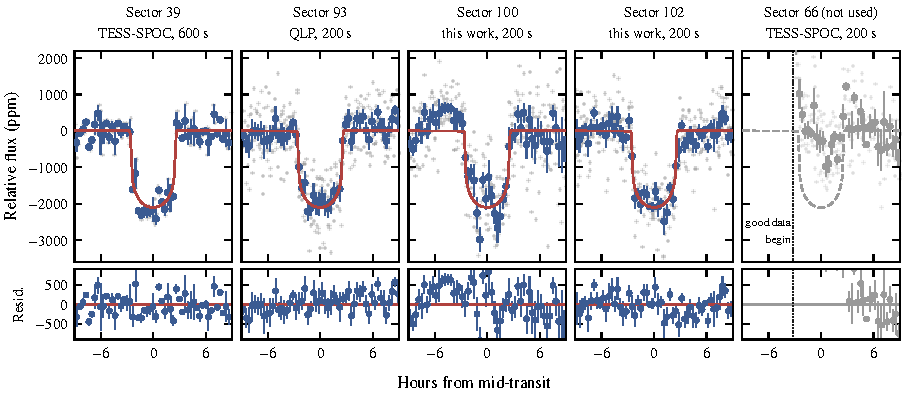
\includegraphics[width=0.92\textwidth]{../../paper/figures/fig1.pdf}
\vspace{-6pt}
\caption{\small The four transits of TIC~402710280.01 (20-min bins) with the median transit model and residuals. The right-hand panel shows the Sector~66 window, lost to scattered light and excluded from all fits \citep{Vora2026}.}
\label{fig:transits}
\end{figure}
\vspace{-12pt}

\renewcommand{\refname}{\large References}
\begingroup\small
\begin{thebibliography}{9}\setlength\itemsep{0pt}
\bibitem[Burke et al.(2020)]{Burke2020} Burke, C.~J., Levine, A., Fausnaugh, M., et al.\ 2020, \texttt{tess-point}, Astrophysics Source Code Library, ascl:2003.001
\bibitem[Giacalone et al.(2021)]{Giacalone2021} Giacalone, S., Dressing, C.~D., Jensen, E.~L.~N., et al.\ 2021, AJ, 161, 24
\bibitem[Vora(2026a)]{Vora2026} Vora, R.\ 2026a, preprint, \href{https://doi.org/10.5281/zenodo.23390317}{doi:10.5281/zenodo.23390317}; data and code, \href{https://doi.org/10.5281/zenodo.23390274}{doi:10.5281/zenodo.23390274}
\bibitem[Vora(2026b)]{PreReg} Vora, R.\ 2026b, pre-registered test of the epoch-57 and 59 transits, \href{https://doi.org/10.5281/zenodo.23390325}{doi:10.5281/zenodo.23390325}
\end{thebibliography}
\endgroup

\end{document}
